\chapter{Subsystems}
\label{chap:subsystems}
.....



\section{Rover}
\label{sec:rover}
...
\section{Structure and Mechanics}
\label{sec:mechanics}
...
\section{Communications and Command and Data-Handling}
\label{sec:comm}
...
\section{Payload}
\label{sec:payload}
...
\section{Thermal Control}
\label{sec:thermalcontrol}
...
\section{Electrical Power System}
\label{sec:EPS}
The EPS (Electrical Power System) is the subsystem responsible for the electrical power supply of INSPIRE. It consists of four funadmental parts, which are the energy source, the PCDU unit (Power Control and Distribution)and the Energy Storage as well as the rover subsystems as the consumers.

\subsection{EPS Budget and Overview}

\begin{figure}[htb]
{\centering
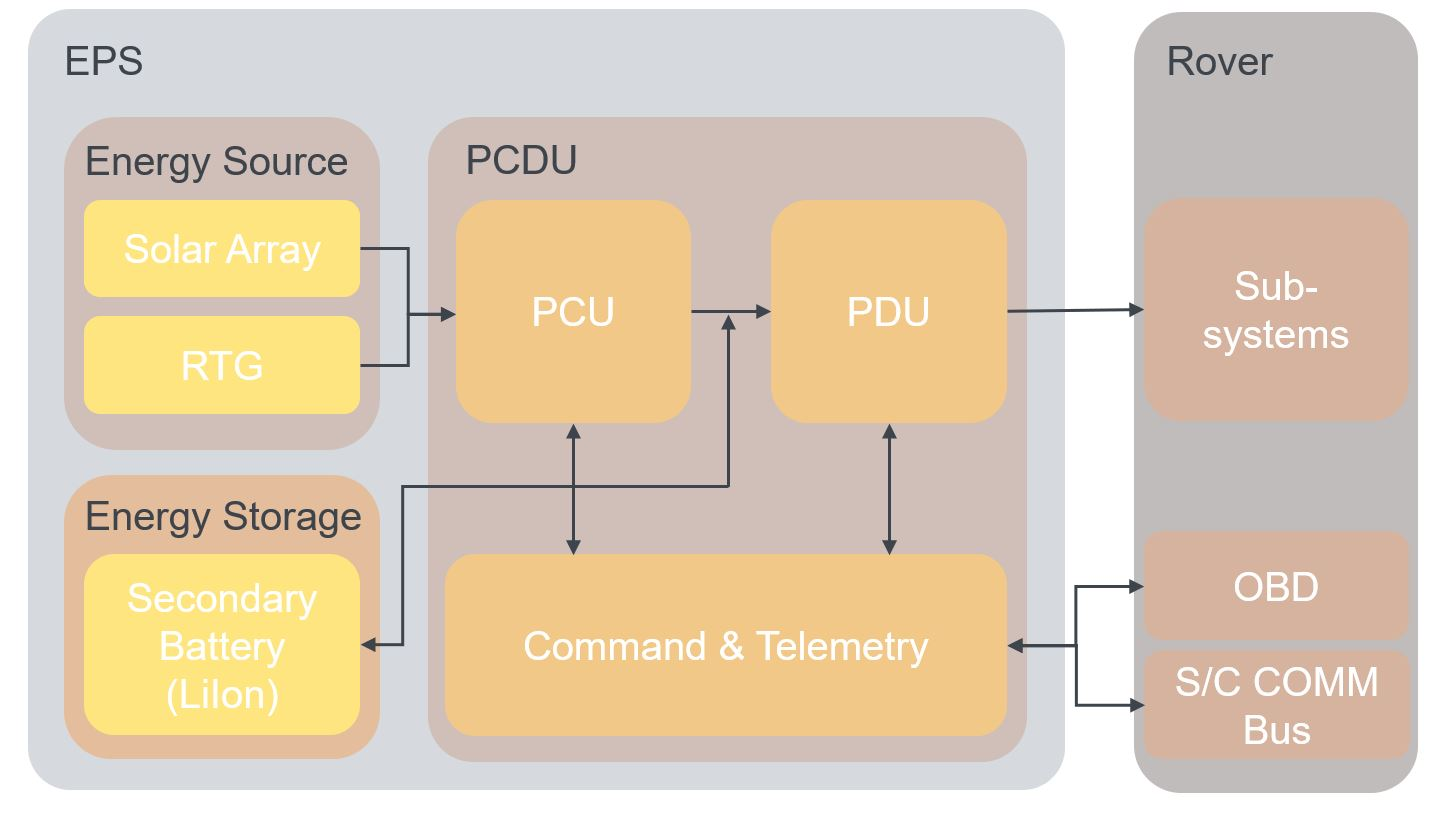
\includegraphics[width=0.5\textwidth]{Media/epsflowchart}
\caption{Functional Flow Chart Diagram for the EPS Subsystem.}
\label{fig:epsflowchart}
}
\end{figure}

\subsection{Energy Source}
For the energy generation of INSPIRE many possible sources were taken into consideration for a trade-off. The outcome of this trade-off is shown in \autoref{fig:epssourcetradeoff} for the most promising energy sources. As a conclusion of this trad-off the decision was made to utilize a Radioisotope Thermoelectric Generator (RTG) as the main energy source for INSPIRE. \\

As the research couldn't find an RTG with a mass suitable for INSPIRE, the solution was to scale down a bigger RTG as an approximation. As a baseline of the scaling the eMMRTG (Enhanced Multi Mission Radioisotope Thermoelectric Generator) was utilized, which is currently under development at NASA and is especially designed for deep space missions like Europa. For the scaling a goal RTG mass of $m_\text{RTG}=3 \ \text{kg}$ was defined and the eMMRTG was scaled down using the given data.
In \autoref{tab:esmmrtg} the scaling results for the eSMMRTG (Enhanced and Scaled Multi Mission Radioisotope Thermoelectric Generator) are listed. The eSMMRTG has a mass of $m_\text{RTG}=3 \ \text{kg}$ and a BOL specific power of $\alpha_\text{BOL}= 4.0 \ \frac{W_{el}}{kg}$ and provides an electrical power of $P_{el} = 12.08 \ W_{el}$ during the mission duration.



\begin{figure}[htb]
{\centering
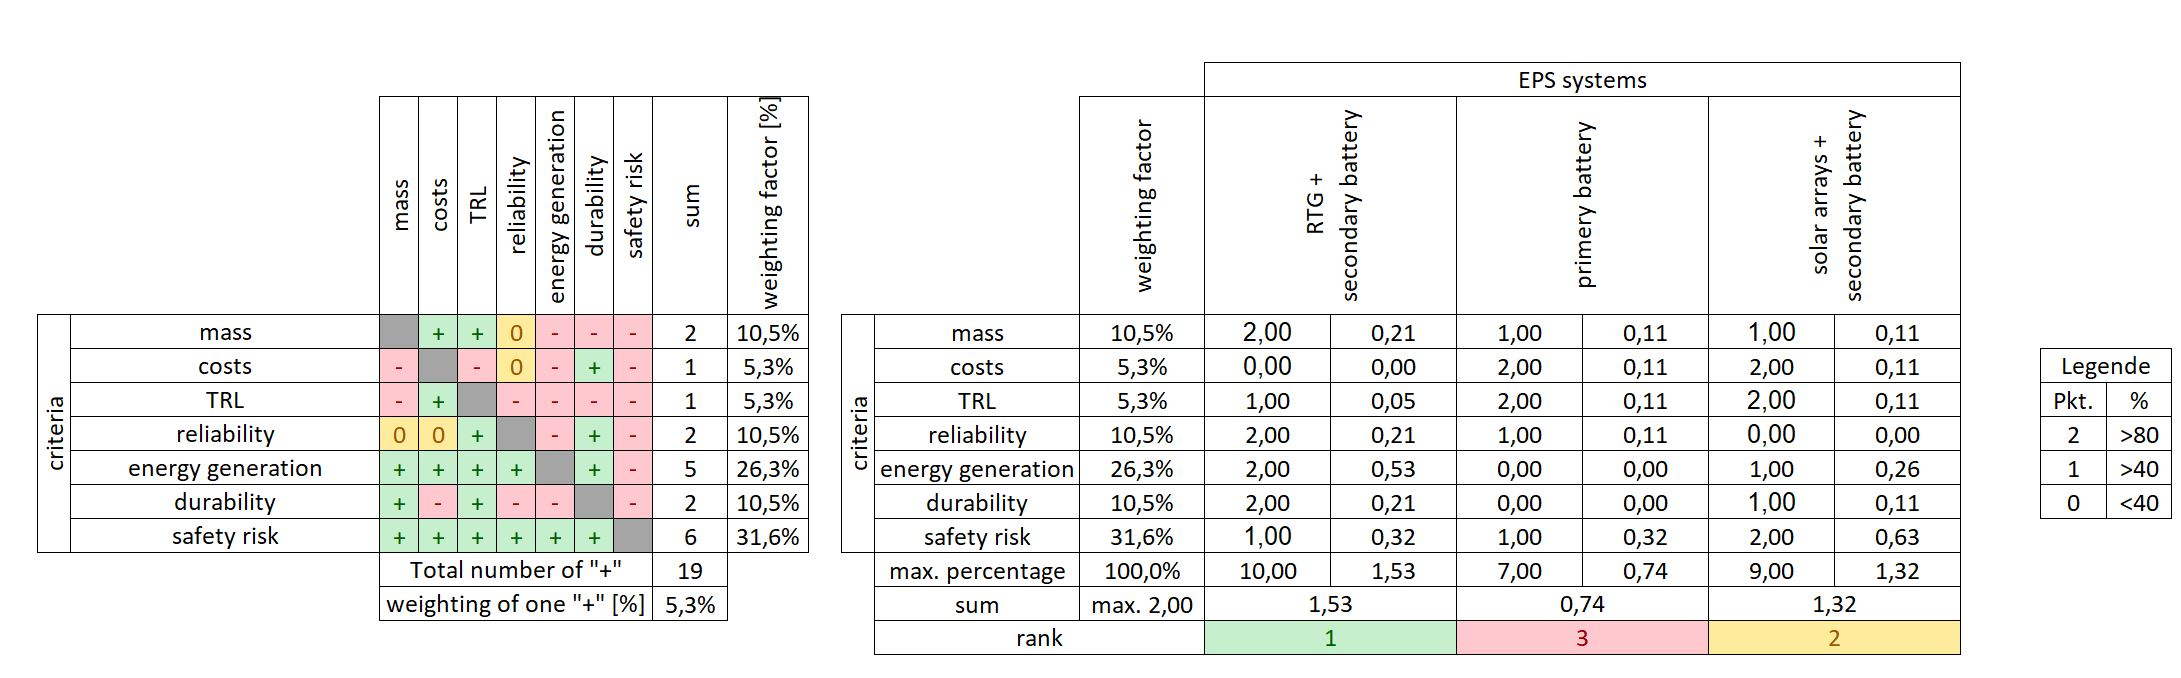
\includegraphics[width=0.7\textwidth]{Media/epssourcetradeoff}
\caption{Trade-Off Conclusion for the EPS Energy Source.}
\label{fig:epssourcetradeoff}
}
\end{figure}

\begin{table}[H]
\centering
\begin{tabular}{|c|c|}
\hline
\multicolumn{2}{|c|}{Scaled eSMMRTG Parameter}                \\ \hline
\textbf{System Mass} $m_\text{RTG}$ [$kg$]                             & \textbf{3.5}     \\ \hline
BOL Specific Power $\alpha_\text{BOL}$ $\frac{W_{el}}{kg}$  & $4.0$     \\ \hline
BOL Power $P_{el,\text{BOL}}$ $\ W_{el}$                    & $14$       \\ \hline
Isotrop                                                     & Pu-238   \\ \hline
Isotrop Half-Life [$a$]                                       & $87.7$     \\ \hline
Flight time and Storage (incl. Margins) [$a$]                 & $7$        \\ \hline
Power Loss Degradation until BOM $\ W_{el}$                 & $0.56$     \\ \hline
BOM Power $P_{el,\text{BOM}}$ $\ W_{el}$                    & $13.44$    \\ \hline
Europa Day Duration [$h$]                                     & $85$       \\ \hline
Mission Duration [$d$]                                        & $106.25$   \\ \hline
End of Mission Power $P_{el,\text{EOM}}$ [$\ W_{el}$]         & $13.42$   \\ \hline
\textbf{Final Power for Study} $P_{el}$ [$\ W_{el}$] (incl. $10\%$ scaling Margin) & \textbf{12.08}    \\ \hline

\end{tabular}
\caption{Parameters for the scaled eSMMRTG based on the eMMRTG.}
\label{tab:esmmrtg}
\end{table}

Furthermore INSPIRE will also be equipped with some radiation hardend solar arrays as already explained in \autoref{subsec:radhard}. Since these solar cells are primarily used for technology testing, the mission must also be able to operate completely without this generated energy. For this reason, and because the expected energy generated by the solar cells is minimal, only the energy generated by the RTG is considered for the Phase 0 Study. However, it should be noted that these solar cells will also generate a certain amount of energy, which will benefit the EPS.


\subsection{Energy Storage} 
For the energy storage of INSPIRE many possible battery types were taken into consideration for a trade-off. As a conclusion of this trad-off the decision was made to utilize LiIon batteries as the secondary batteries of INSPIRE. This decision is primarly based on LiIon batteries high energy density, temperature range, robust performance and long operating and cycle life in extreme environemnts. \\
As the RTG only generates a small constant power the main energy source during the mission will be the accumulated energy of the batteries. The rover will charge the batteries at night, so the next exploration day can start with full capacity. Furthermore the batteries have to be charged during day time to maintain operations.\\

For the sizing of the batteries, the rover motion was chosen as the design driver, since this is the highest energy consuming state of the rover and additionally mission critical for INSPIRE. The rover motion consists of an interaction of the Locomotion and Perception mode as already mentioned in \autoref{chap:Operation}. Therefore it was defined that INSPIRE shall be able to drive $ 50 \ m $ (including alternating Locomotion and Perception Mode) with a fully charged Battery. The required Battery Capacity $C_\text{Batt,req}$ can be caculated using \autoref{eq:batreq}. The results are listed in \autoref{tab:batsize}.


\begin{equation}
C_\text{Batt} = \frac{P_\text{el,req} \cdot t_e }{DoD \cdot \eta_\text{LiIon}}
\label{eq:batreq}
\end{equation}

\begin{table}[htb]
\centering
\resizebox{\textwidth}{!}{%
\begin{tabular}{|l|c|c|}
\hline
\textbf{Power Consumption Mode:}                        & \textbf{Locomotion} & \textbf{Perception} \\ \hline
Required Electrical Power $P_\text{el,req}$ [$W_{el}$]         & 283.43              & 14.01               \\ \hline
Duration of the mode$ t_e$ [$s$]                          & 500              & 15000            \\ \hline
$DOD$ for Dimensioning [-]                              & 0.90                & 0.90                \\ \hline
Efficiency of LiIon Cells $\eta_\text{LiIon}$ [-]       & 0.95                & 0.95                \\ \hline
Required Battery Capacity per mode $C_\text{mode}$ [$Wh$] & 46.04               & 68.27               \\ \hline
\textbf{Total Required Battery Capacity} $C_\text{Batt,req}$ [$Wh$]    & \multicolumn{2}{c|}{\textbf{114.32}}               \\ \hline
\end{tabular}%
}
\caption{Power consumption mode used as design case for the battery sizing.}
\label{tab:batsize}
\end{table}

Using these values a suitable battery cell and battery design configuration were conducted. Using these parameters the battery capacity $C_\text{Batt}$ can be calcuated:

\begin{equation}
C_\text{Batt} = C_\text{cell} \cdot V_\text{cell} \cdot N \cdot M .
\label{eq:batuse}
\end{equation}

According to the ECSS reliability restrictions 1 battery string must be substracted for dimensionsing. Furthermore a $30 \%$ margin on the energy content was applied. This leads to a final battery configuration with a capacity of $C_\text{Batt}=138,88 \ Wh$ and a mass of $m = 1980 \ g$. The final battery values are listed in \autoref{eq:batuse}.


% Please add the following required packages to your document preamble:
% \usepackage{graphicx}
\begin{table}[htb]
\centering
\resizebox{\textwidth}{!}{%
\begin{tabular}{|c|c|}
\hline
\multicolumn{2}{|c|}{\textbf{SAFT 176065 xlr}}                                                                \\ \hline
\multicolumn{2}{|c|}{\textbf{Configuration:}}                                                                 \\ \hline
Battery Configuration                                                           & $4s3p$                        \\ \hline
Cells in Sereis $s$ N [-]                                                       & $4$                           \\ \hline
Cells in Parallel $p$ M [-]                                                     & $3$                           \\ \hline
\multicolumn{2}{|c|}{\textbf{Cell Parameters:}}                                                               \\ \hline
Typical Cell Capacity   [$Ah$]                                                    & $6.8$                         \\ \hline
Nominal Cell Voltage [$V$]                                                        & $3.65$                        \\ \hline
Nominal Cell Capacity [$Wh$]                                                      & $24.8$                        \\ \hline
Typical Cell Mass [$kg$]                                                          & $0.15$                        \\ \hline
Energy Density [$Wh/kg$]                                                     & $165.33$                      \\ \hline
\multicolumn{2}{|c|}{\textbf{Actual Battery Configuration Parameters:}}                                       \\ \hline
Battery Voltage $V_\text{Batt}$ [V]                                             & $14.6$                        \\ \hline
Battery Nominal Capacity $E_\text{Batt}$ [$Wh$]                                   & $297.6$                       \\ \hline
Battery Mass [$kg$]                                                               & $1.8$                         \\ \hline
\textbf{Battery Mass} (incl. $10\%$ Margin) [$kg$]                                         & \textbf{1.98}                        \\ \hline
\multicolumn{2}{|c|}{\textbf{Configruation according to ECSS reliability restrictions and margins included:}} \\ \hline
Battery Configuration                                                           & $4s2p$                        \\ \hline
Cells in Sereis $s$ N [-]                                                       & $4$                           \\ \hline
Cells in Parallel $p$ M [-]                                                     & $2$                           \\ \hline
Battery Voltage $V_\text{Batt}$ [$V$]                                             & $14.6 $                       \\ \hline
Battery Nominal Capacity $E_\text{Batt}$ [$Wh$]                                   & $198.4$                       \\ \hline
$30\%$ Margin on Energy Content                                                 & $0.3$                         \\ \hline
\textbf{Battery Nominal Capacity} $E_\text{Batt}$ incl. Margin [$Wh$]                      & \textbf{138.88}                      \\ \hline
Useable Energy Density [$Wh/kg$]                                              & $70.14$                       \\ \hline
\end{tabular}%
}
\caption{INSPIRE battery parameters.}
\label{tab:battery}
\end{table}


\subsection{EPS Power Control and Distribution}
In order to ensure the full functionality of the EPS, the last main component to be selected is a suitable PCDU. As described in \autoref{fig:epsflowchart}, the PCDU forms the heart of the EPS and is also an important interface to the OBC and COMM. Furthermore the PCDU shall be able to monitor and control the rover system if necessary through watchdogs, HPC (High Priority Commands) and direct connections to the OBC and COMM.\\
The PCDU has the challenging task not only to process the RTG as the main energy source, but also to process solar cells as secondary energy sources. Therefore, a PCDU was sought which has the required size, dimensions and range of functions. The research resulted in the Nova PCDU from Bradford DSI. In addition, margins were added to the PCDU to ensure feasibility.

\clearpage

\section{Radiation}
\label{sec:Radiation}

Compared to the radiation environment near Earth the radiation environment near Jupiter is multiple times stronger. It has the highest radiation levels of any planet in our solar systems \cite{Platzhalter}. In order to survive these harsh environmental conditions, special emphasis must be placed on the radiation protection. In \autoref{fig:trappedprotonelectronfluxes}, the average trapped proton and electron fluxes on Europa's orbit around Jupiter are shown in comparison to the outer Van Allen radiation belt around Earth. However, in contrast to the Van Allen radiation belt, the duration within the radiation environment on Europa cannot be minimised and the rover has to be designed to withstand the entire mission duration of 30 days. \\ \\
In oder to design and evaluate different radiation protection approaches, different calculations have to be performed. For this purpose the ESA SPace ENVironment Information System (SPENVIS) is used \cite{Platzhalter}. All calculations and figures in \autoref{sec:Radiation} are performed with SPENVIS unless otherwise stated.

\subsection{Radiation Protection}

Various options are available to protect the rover against the radiation. A common approach is the use of aluminium or titanium as these materials can also act as structural elements. However, due to the mass constraints of 30 kg other materials or material compositions are taken in consideration which are more mass effective. In \autoref{tab:OptimalRadiationProtection}, an optimised shield structure is presented for different weight thresholds designed for the radiation environment around Jupiter.

\begin{wraptable}{r}{8cm}
\centering
\caption{Optimal shield structure for an Jupiter mission. \cite{Platzhalter}}
\begin{adjustbox}{max width=\textwidth}
\begin{tabular}[l]{cccccc}

	\toprule
	
	Areal Density	&	\(0.5\)	&	\(1\) &  \(2\) & \(3\)	\\
	/ \(\text{g/cm}^2\)	&	&	&  & \\
	
	\midrule
	
	
	Layer No. 1	&	Pb &  Pb & W	& Ta	\\
	/ mm	&	0.415 &  0.829 & 0.984	& 1.563	\\
	
	
	Layer No. 2	&	Fe	&  Mg &	Mg & Al \\
	/ mm	&	\(0.033\)	&  \(0.158\) &	\(0.540\) & \(0.399\) \\
	
	
	Layer No. 3 &	-	&  -	& - & Mg \\
	/ mm &	-	&  -	& - & \(0.150\) \\
	

	\bottomrule

\end{tabular}
\end{adjustbox}
\label{tab:OptimalRadiationProtection}
\end{wraptable}

The difference between an aluminium or titanium shielding and an optimised structure listed in \autoref{tab:OptimalRadiationProtection} for the total ionizing dose (TID) is shown in \autoref{fig:AluminiumTitanOptimised}. \\ \\
Due to the mass savings of the optimised structure it will be used where the radiation protection of the aluminium structure is not sufficient. In order to reduce the mass further, a radiation vault is utilised that highly sensible components do not have to be shielded separately.

\subsection{Components}

%TODO Auswahl 0.5 g/cm^2

Every component on the rover has a different radiation tolerance and therefore have to be placed at different compartments within the rover. The radiation tolerances are listed in \autoref{tab:RadiationList}.

\subsection{Improvements}

\subsection{Conclusion}

\clearpage

\section{Locomotion}
\label{sec:locomotion}



\section{Control and Autonomy}
\label{sec:ControlandAutonomy}

\cleardoublepage